\chapter{Arithmetic: The Construction of Number Systems}

\section{From Sets to Numbers}

\begin{intuition}
We've built natural numbers as sets:
\[0 = \emptyset, \quad 1 = \{0\}, \quad 2 = \{0, 1\}, \quad 3 = \{0, 1, 2\}, \ldots\]

But what does ``$2 + 3$'' mean? What does ``$2 \times 3$'' mean?

These operations aren't \textit{given}---we must \textbf{define} them rigorously from scratch.

This chapter constructs the familiar number systems ($\mathbb{N}, \mathbb{Z}, \mathbb{Q}$) and proves all their arithmetic properties from set-theoretic foundations.
\end{intuition}

\vspace{0.5em}

\begin{historicalnote}
\textbf{The Arithmetization of Mathematics}

Before the 19th century, arithmetic was considered self-evident. But a crisis emerged:

\textbf{Ancient Greeks}: Discovered irrational numbers like $\sqrt{2}$, causing philosophical turmoil.

\textbf{19th Century Crisis}:
\begin{itemize}
    \item Analysts used real numbers freely but couldn't define them rigorously
    \item Dedekind (1858): ``What are numbers and what should they be?''
    \item Dedekind cuts (1872): Constructed $\mathbb{R}$ from $\mathbb{Q}$
    \item Cantor (1872): Alternative construction via Cauchy sequences
    \item Peano (1889): Axiomatized natural numbers
    \item Frege, Russell: Attempted to reduce arithmetic to pure logic (Logicism)
\end{itemize}

\textbf{Zermelo-Fraenkel Set Theory (1908-1922)}: Provided the ultimate foundation---all numbers are sets, all operations are functions (which are sets).

Today's approach: Define $\mathbb{N}$ via von Neumann ordinals, then construct $\mathbb{Z}, \mathbb{Q}, \mathbb{R}$ as successive extensions.
\end{historicalnote}

\section{Arithmetic on Natural Numbers}

We've defined natural numbers using the Axiom of Infinity:
\[0 := \emptyset, \quad S(n) := n \cup \{n\} \quad \text{(successor function)}\]

Now we define addition and multiplication.

\subsection{The Principle of Mathematical Induction}

Before defining operations, we must establish our primary tool for proving statements about natural numbers: \textbf{Induction}.

Recall that $\mathbb{N}$ is defined as the smallest inductive set (by the Axiom of Infinity). This gives us the following principle:

\begin{theorem}[Principle of Mathematical Induction]
Let $P(n)$ be a property involving a natural number $n$. If:
\begin{enumerate}
    \item \textbf{Base Case}: $P(0)$ is true, and
    \item \textbf{Inductive Step}: For all $k \in \mathbb{N}$, if $P(k)$ is true, then $P(S(k))$ is true,
\end{enumerate}
then $P(n)$ is true for all $n \in \mathbb{N}$.
\end{theorem}

\begin{intuition}
This works like dominoes:
\begin{itemize}
    \item Base case: You knock over the first domino (0).
    \item Inductive step: Each domino knocks over the next one ($k \implies S(k)$).
    \item Conclusion: All dominoes fall.
\end{itemize}
Because $\mathbb{N}$ contains \textit{only} elements reached this way (it's the \textit{smallest} inductive set), the property holds for all numbers.
\end{intuition}

\subsection{Addition}

\begin{definition}[Addition on $\mathbb{N}$]
For $m, n \in \mathbb{N}$, define $m + n$ recursively:

\textbf{Base case}: $m + 0 := m$

\textbf{Recursive case}: $m + S(n) := S(m + n)$

In other notation: $m + (n+1) = (m+n) + 1$
\end{definition}

\begin{example}
Let's compute $2 + 3$ from the definition:
\begin{align*}
2 + 3 &= 2 + S(2) \\
&= S(2 + 2) \quad \text{(by recursive case)} \\
&= S(2 + S(1)) \\
&= S(S(2 + 1)) \\
&= S(S(2 + S(0))) \\
&= S(S(S(2 + 0))) \\
&= S(S(S(2))) \quad \text{(by base case)} \\
&= S(S(3)) \\
&= S(4) \\
&= 5
\end{align*}
\end{example}

\begin{center}
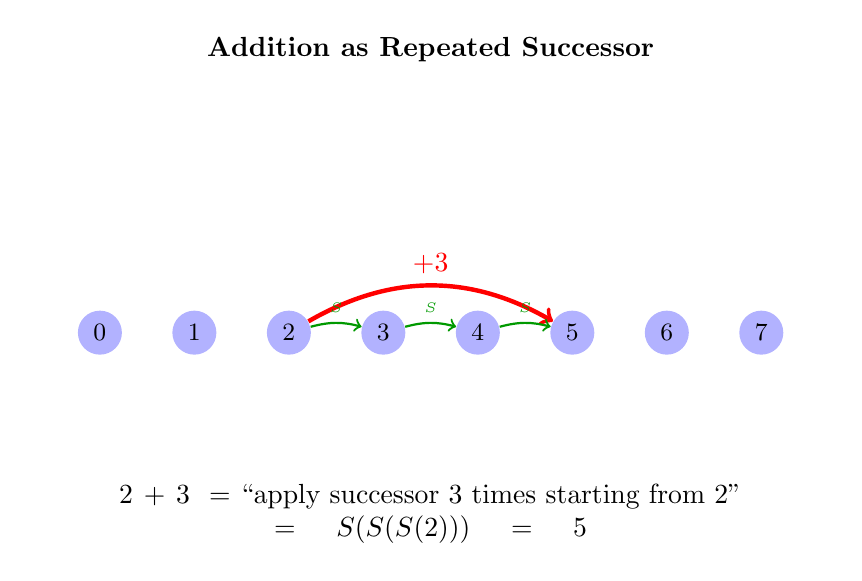
\begin{tikzpicture}[scale=1.2]
    \node at (3.5, 5) {\textbf{Addition as Repeated Successor}};
    
    % Number line
    \foreach \x in {0,...,7} {
        \node[circle, fill=blue!30, inner sep=3pt] (n\x) at (\x, 2) {\small $\x$};
    }
    
    % Arrows showing 2 + 3
    \draw[->, ultra thick, red, bend left=30] (n2) to node[above] {$+3$} (n5);
    
    \draw[->, thick, green!60!black] (n2) to[bend left=15] node[above] {\tiny $S$} (n3);
    \draw[->, thick, green!60!black] (n3) to[bend left=15] node[above] {\tiny $S$} (n4);
    \draw[->, thick, green!60!black] (n4) to[bend left=15] node[above] {\tiny $S$} (n5);
    
    \node[below, text width=10cm, align=center] at (3.5, 0.5) {
        $2 + 3 =$ ``apply successor 3 times starting from 2'' \\
        $= S(S(S(2))) = 5$
    };
\end{tikzpicture}
\end{center}

\begin{theorem}[Properties of Addition]
For all $m, n, p \in \mathbb{N}$:
\begin{enumerate}
    \item \textbf{Right Identity}: $n + 0 = n$
    \item \textbf{Left Identity}: $0 + n = n$
    \item \textbf{Commutativity}: $m + n = n + m$
    \item \textbf{Associativity}: $(m + n) + p = m + (n + p)$
\end{enumerate}
\end{theorem}

\begin{proof}
\textbf{(1) Right Identity}: By definition, $n + 0 = n$. $\checkmark$

\textbf{(2) Left Identity}: Prove by induction on $n$.

\textit{Base case}: $0 + 0 = 0$ (by definition). $\checkmark$

\textit{Inductive step}: Assume $0 + n = n$ (IH). Show $0 + S(n) = S(n)$.
\begin{align*}
0 + S(n) &= S(0 + n) \quad \text{(by definition of addition)} \\
&= S(n) \quad \text{(by IH)}
\end{align*}
Therefore $0 + S(n) = S(n)$. By induction, $0 + n = n$ for all $n$. $\checkmark$

\textbf{(3) Commutativity}: First prove a lemma.

\textbf{Lemma}: $S(m) + n = S(m + n)$ for all $m, n$.

\textit{Proof of Lemma}: Induction on $n$.

\textit{Base}: $S(m) + 0 = S(m) = S(m + 0)$. $\checkmark$

\textit{Step}: Assume $S(m) + n = S(m + n)$ (IH).
\begin{align*}
S(m) + S(n) &= S(S(m) + n) \quad \text{(definition)} \\
&= S(S(m + n)) \quad \text{(IH)} \\
&= S(m + S(n)) \quad \text{(definition)}
\end{align*}
Lemma proved. $\checkmark$

Now prove commutativity by induction on $n$.

\textit{Base}: $m + 0 = m = 0 + m$ (by right and left identity). $\checkmark$

\textit{Step}: Assume $m + n = n + m$ (IH). Show $m + S(n) = S(n) + m$.
\begin{align*}
m + S(n) &= S(m + n) \quad \text{(definition)} \\
&= S(n + m) \quad \text{(IH)} \\
&= S(n) + m \quad \text{(Lemma)}
\end{align*}
Therefore addition is commutative. $\checkmark$

\textbf{(4) Associativity}: Prove by induction on $p$.

\textit{Base}: $(m + n) + 0 = m + n = m + (n + 0)$. $\checkmark$

\textit{Step}: Assume $(m + n) + p = m + (n + p)$ (IH).
\begin{align*}
(m + n) + S(p) &= S((m + n) + p) \quad \text{(definition)} \\
&= S(m + (n + p)) \quad \text{(IH)} \\
&= m + S(n + p) \quad \text{(definition)} \\
&= m + (n + S(p)) \quad \text{(definition)}
\end{align*}
Therefore addition is associative. $\checkmark$
\end{proof}

\subsection{Multiplication}

\begin{definition}[Multiplication on $\mathbb{N}$]
For $m, n \in \mathbb{N}$, define $m \cdot n$ (or $m \times n$) recursively:

\textbf{Base case}: $m \cdot 0 := 0$

\textbf{Recursive case}: $m \cdot S(n) := m \cdot n + m$

In other notation: $m \cdot (n+1) = m \cdot n + m$
\end{definition}

\begin{keyidea}
Multiplication is \textbf{repeated addition}:
\[m \cdot n = \underbrace{m + m + \cdots + m}_{n \text{ times}}\]

For example:
\[3 \cdot 4 = 3 + 3 + 3 + 3 = 12\]
\end{keyidea}

\begin{example}
Compute $3 \cdot 2$ from the definition:
\begin{align*}
3 \cdot 2 &= 3 \cdot S(1) \\
&= 3 \cdot 1 + 3 \\
&= 3 \cdot S(0) + 3 \\
&= (3 \cdot 0 + 3) + 3 \\
&= (0 + 3) + 3 \quad \text{(by base case)} \\
&= 3 + 3 \\
&= 6
\end{align*}
\end{example}

\begin{center}
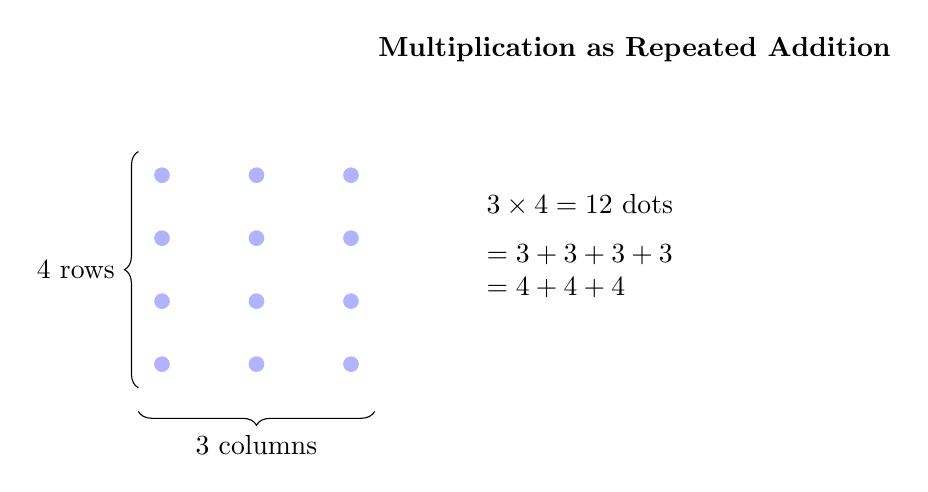
\begin{tikzpicture}[scale=1.0]
    \node at (6, 4) {\textbf{Multiplication as Repeated Addition}};
    
    % Visual representation of 3 × 4
    \foreach \y in {0,1,2,3} {
        \foreach \x in {0,1,2} {
            \node[circle, fill=blue!30, inner sep=2pt] at (\x*1.2, \y*0.8) {};
        }
    }
    
    \draw[decorate, decoration={brace, amplitude=5pt}] (-0.3, -0.3) -- (-0.3, 2.7) node[midway, left=5pt] {4 rows};
    \draw[decorate, decoration={brace, amplitude=5pt, mirror}] (-0.3, -0.6) -- (2.7, -0.6) node[midway, below=5pt] {3 columns};
    
    \node[right, text width=5cm] at (4, 1.5) {
        $3 \times 4 = 12$ dots \\[0.2cm]
        $= 3 + 3 + 3 + 3$ \\
        $= 4 + 4 + 4$
    };
\end{tikzpicture}
\end{center}

\begin{theorem}[Properties of Multiplication]
For all $m, n, p \in \mathbb{N}$:
\begin{enumerate}
    \item \textbf{Right Zero}: $n \cdot 0 = 0$
    \item \textbf{Left Zero}: $0 \cdot n = 0$
    \item \textbf{Right Identity}: $n \cdot 1 = n$
    \item \textbf{Left Identity}: $1 \cdot n = n$
    \item \textbf{Commutativity}: $m \cdot n = n \cdot m$
    \item \textbf{Associativity}: $(m \cdot n) \cdot p = m \cdot (n \cdot p)$
    \item \textbf{Distributivity}: $m \cdot (n + p) = m \cdot n + m \cdot p$
\end{enumerate}
\end{theorem}

\begin{proof}
\textbf{(1) Right Zero}: By definition, $n \cdot 0 = 0$. $\checkmark$

\textbf{(2) Left Zero}: Induction on $n$.

\textit{Base}: $0 \cdot 0 = 0$ (definition). $\checkmark$

\textit{Step}: Assume $0 \cdot n = 0$ (IH).
\begin{align*}
0 \cdot S(n) &= 0 \cdot n + 0 \quad \text{(definition)} \\
&= 0 + 0 \quad \text{(IH)} \\
&= 0
\end{align*}
$\checkmark$

\textbf{(3) Right Identity}: 
\begin{align*}
n \cdot 1 &= n \cdot S(0) \\
&= n \cdot 0 + n \\
&= 0 + n \\
&= n
\end{align*}
$\checkmark$

\textbf{(4) Left Identity}: Induction on $n$.

\textit{Base}: $1 \cdot 0 = 0$ (by definition). This matches $n=0$. $\checkmark$

\textit{Step}: Assume $1 \cdot n = n$ (IH). Show $1 \cdot S(n) = S(n)$.
\begin{align*}
1 \cdot S(n) &= 1 \cdot n + 1 \quad \text{(definition)} \\
&= n + 1 \quad \text{(IH)} \\
&= S(n)
\end{align*}
Therefore $1 \cdot n = n$ for all $n$. $\checkmark$

\textbf{(5) Commutativity}: First prove lemmas.

\textbf{Lemma 1}: $S(m) \cdot n = m \cdot n + n$

\textit{Proof}: Induction on $n$.

\textit{Base}: $S(m) \cdot 0 = 0 = 0 + 0 = m \cdot 0 + 0$. $\checkmark$

\textit{Step}: Assume $S(m) \cdot n = m \cdot n + n$ (IH).
\begin{align*}
S(m) \cdot S(n) &= S(m) \cdot n + S(m) \quad \text{(def)} \\
&= (m \cdot n + n) + S(m) \quad \text{(IH)} \\
&= m \cdot n + (n + S(m)) \\
&= m \cdot n + (S(m) + n) \quad \text{(commutativity of +)} \\
&= m \cdot n + (m + S(n)) \\
&= (m \cdot n + m) + S(n) \\
&= m \cdot S(n) + S(n)
\end{align*}
Lemma 1 proved. $\checkmark$

Now prove commutativity by induction on $n$.

\textit{Base}: $m \cdot 0 = 0 = 0 \cdot m$ (by left and right zero). $\checkmark$

\textit{Step}: Assume $m \cdot n = n \cdot m$ (IH).
\begin{align*}
m \cdot S(n) &= m \cdot n + m \quad \text{(def)} \\
&= n \cdot m + m \quad \text{(IH)} \\
&= S(n) \cdot m \quad \text{(Lemma 1)}
\end{align*}
$\checkmark$

\textbf{(6) Associativity}: Prove by induction on $p$.

\textit{Base}: $(m \cdot n) \cdot 0 = 0 = m \cdot 0 = m \cdot (n \cdot 0)$. $\checkmark$

\textit{Step}: Assume $(m \cdot n) \cdot p = m \cdot (n \cdot p)$ (IH).
\begin{align*}
(m \cdot n) \cdot S(p) &= (m \cdot n) \cdot p + (m \cdot n) \quad \text{(def)} \\
&= m \cdot (n \cdot p) + (m \cdot n) \quad \text{(IH)} \\
&= m \cdot (n \cdot p + n) \quad \text{(distributivity, proved next)} \\
&= m \cdot (n \cdot S(p))
\end{align*}
$\checkmark$

\textbf{(7) Distributivity}: Prove by induction on $p$.

\textit{Base}: $m \cdot (n + 0) = m \cdot n = m \cdot n + 0 = m \cdot n + m \cdot 0$. $\checkmark$

\textit{Step}: Assume $m \cdot (n + p) = m \cdot n + m \cdot p$ (IH).
\begin{align*}
m \cdot (n + S(p)) &= m \cdot S(n + p) \\
&= m \cdot (n + p) + m \quad \text{(def)} \\
&= (m \cdot n + m \cdot p) + m \quad \text{(IH)} \\
&= m \cdot n + (m \cdot p + m) \quad \text{(associativity of +)} \\
&= m \cdot n + m \cdot S(p) \quad \text{(def)}
\end{align*}
$\checkmark$
\end{proof}

\begin{remark}
These proofs are tedious but essential---we've just proved that $\mathbb{N}$ with $+$ and $\cdot$ satisfies the axioms of a \textbf{commutative semiring}.

The structure $(\mathbb{N}, +, \cdot, 0, 1)$ is the \textbf{free} commutative semiring on one generator.
\end{remark}

\section{The Integers: $\mathbb{Z}$}

\begin{intuition}
Natural numbers are insufficient: the equation $x + 3 = 2$ has no solution in $\mathbb{N}$.

We need \textbf{negative numbers} to solve equations like $x + a = b$ for any $a, b$.

How do we construct negatives from sets? We can't just ``add them''---we must build them systematically.
\end{intuition}

\subsection{Construction of $\mathbb{Z}$}

\begin{definition}[Integers as Pairs]
Define an equivalence relation on $\mathbb{N} \times \mathbb{N}$:
\[(m, n) \sim (p, q) \iff m + q = p + n\]

The \textbf{integers} are the equivalence classes:
\[\mathbb{Z} := (\mathbb{N} \times \mathbb{N}) / {\sim}\]

We write $[(m, n)]$ for the equivalence class of $(m, n)$.
\end{definition}

\begin{keyidea}
\textbf{Interpretation}: The pair $(m, n)$ represents the ``difference'' $m - n$.

\begin{itemize}
    \item $[(3, 0)]$ represents $3 - 0 = 3$ (positive)
    \item $[(0, 5)]$ represents $0 - 5 = -5$ (negative)
    \item $[(7, 4)]$ represents $7 - 4 = 3$ (same as $[(3, 0)]$)
    \item $[(2, 2)]$ represents $2 - 2 = 0$ (zero)
\end{itemize}

The equivalence relation says: $(m, n) \sim (p, q)$ if $m - n = p - q$ (informally).

Formally: $m + q = p + n$ (avoiding subtraction, which we haven't defined yet!)
\end{keyidea}

\begin{theorem}
The relation $\sim$ is an equivalence relation.
\end{theorem}

\begin{proof}
\textbf{Reflexive}: $(m, n) \sim (m, n)$ because $m + n = m + n$. $\checkmark$

\textbf{Symmetric}: If $(m, n) \sim (p, q)$, then $m + q = p + n$, so $p + n = m + q$, thus $(p, q) \sim (m, n)$. $\checkmark$

\textbf{Transitive}: If $(m, n) \sim (p, q)$ and $(p, q) \sim (r, s)$, then:
\[m + q = p + n \quad \text{and} \quad p + s = r + q\]

Adding these equations:
\[m + q + p + s = p + n + r + q\]

Cancel $p$ and $q$ (using cancellation law for natural numbers):
\[m + s = r + n\]

Therefore $(m, n) \sim (r, s)$. $\checkmark$
\end{proof}

\begin{center}
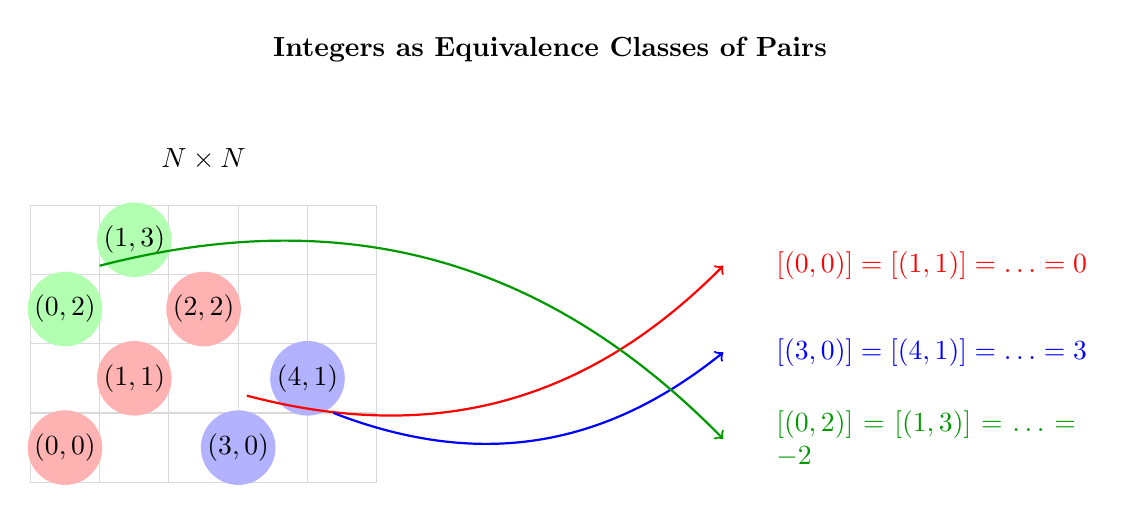
\begin{tikzpicture}[scale=1.1]
    \node at (6, 5) {\textbf{Integers as Equivalence Classes of Pairs}};
    
    % Grid showing pairs
    \draw[step=0.8, gray!30] (0,0) grid (4,3.2);
    
    \node[above] at (2, 3.5) {$\mathbb{N} \times \mathbb{N}$};
    
    % Examples
    \node[fill=red!30, circle, inner sep=1pt] at (0.4, 0.4) {$(0,0)$};
    \node[fill=red!30, circle, inner sep=1pt] at (1.2, 1.2) {$(1,1)$};
    \node[fill=red!30, circle, inner sep=1pt] at (2.0, 2.0) {$(2,2)$};
    
    \node[fill=blue!30, circle, inner sep=1pt] at (2.4, 0.4) {$(3,0)$};
    \node[fill=blue!30, circle, inner sep=1pt] at (3.2, 1.2) {$(4,1)$};
    
    \node[fill=green!30, circle, inner sep=1pt] at (0.4, 2.0) {$(0,2)$};
    \node[fill=green!30, circle, inner sep=1pt] at (1.2, 2.8) {$(1,3)$};
    
    % Arrows showing equivalence classes
    \draw[->, thick, red] (2.5, 1) to[bend right] (8, 2.5);
    \draw[->, thick, blue] (3.5, 0.8) to[bend right] (8, 1.5);
    \draw[->, thick, green!60!black] (0.8, 2.5) to[bend left] (8, 0.5);
    
    % Integer labels
    \node[right, text width=4cm] at (8.5, 2.5) {
        \textcolor{red}{$[(0,0)] = [(1,1)] = \ldots = 0$}
    };
    \node[right, text width=4cm] at (8.5, 1.5) {
        \textcolor{blue}{$[(3,0)] = [(4,1)] = \ldots = 3$}
    };
    \node[right, text width=4cm] at (8.5, 0.5) {
        \textcolor{green!60!black}{$[(0,2)] = [(1,3)] = \ldots = -2$}
    };
\end{tikzpicture}
\end{center}

\subsection{Arithmetic on $\mathbb{Z}$}

\begin{definition}[Operations on $\mathbb{Z}$]
Define addition and multiplication on equivalence classes:

\textbf{Addition}: $[(m, n)] + [(p, q)] := [(m + p, n + q)]$

\textbf{Multiplication}: $[(m, n)] \cdot [(p, q)] := [(mp + nq, mq + np)]$

\textbf{Negation}: $-[(m, n)] := [(n, m)]$

\textbf{Embedding}: $\iota: \mathbb{N} \to \mathbb{Z}$ by $\iota(n) = [(n, 0)]$
\end{definition}

\begin{theorem}[The Embedding $\mathbb{N} \hookrightarrow \mathbb{Z}$]
The map $\iota: \mathbb{N} \to \mathbb{Z}$ defined by $\iota(n) = [(n, 0)]$ is an injective homomorphism that preserves addition, multiplication, and order. This allows us to view $\mathbb{N}$ as a subset of $\mathbb{Z}$.
\end{theorem}

\begin{proof}
We verify the required properties:

\textbf{(1) Well-defined:} For any $n \in \mathbb{N}$, we have $\iota(n) = [(n, 0)] \in \mathbb{Z}$ (an equivalence class). $\checkmark$

\textbf{(2) Injective:} Suppose $\iota(m) = \iota(n)$ for $m, n \in \mathbb{N}$.

Then $[(m, 0)] = [(n, 0)]$, which means $(m, 0) \sim (n, 0)$.

By definition of $\sim$, this means $m + 0 = n + 0$, so $m = n$. $\checkmark$

\textbf{(3) Preserves Addition:}
\begin{align*}
\iota(m + n) &= [(m + n, 0)] \\
&= [(m, 0)] + [(n, 0)] \quad \text{(by definition of $+$ on $\mathbb{Z}$)} \\
&= \iota(m) + \iota(n)
\end{align*}
$\checkmark$

\textbf{(4) Preserves Multiplication:}
\begin{align*}
\iota(m \cdot n) &= [(mn, 0)] \\
&= [(m \cdot n + 0 \cdot 0, m \cdot 0 + 0 \cdot n)] \\
&= [(m, 0)] \cdot [(n, 0)] \quad \text{(by definition of $\cdot$ on $\mathbb{Z}$)} \\
&= \iota(m) \cdot \iota(n)
\end{align*}
$\checkmark$

\textbf{(5) Preserves Order:} Recall that on $\mathbb{N}$, we have $m < n$ iff $\exists k \in \mathbb{N}, m + k = n$ with $k \neq 0$.

On $\mathbb{Z}$, we define $[(a, b)] < [(c, d)]$ iff $a + d < b + c$ in $\mathbb{N}$.

Now suppose $m < n$ in $\mathbb{N}$, so $m + k = n$ for some $k > 0$.

Then:
\begin{align*}
\iota(m) = [(m, 0)] &\quad \text{and} \quad \iota(n) = [(n, 0)] = [(m + k, 0)]
\end{align*}

To check $[(m, 0)] < [(m + k, 0)]$ in $\mathbb{Z}$:
\[m + 0 < 0 + (m + k) = m + k \quad \text{in } \mathbb{N}\]

This holds since $k > 0$. $\checkmark$

Conversely, if $\iota(m) < \iota(n)$, then $[(m, 0)] < [(n, 0)]$, so $m + 0 < 0 + n$, hence $m < n$ in $\mathbb{N}$. $\checkmark$

Therefore $\iota$ is an order-preserving ring homomorphism, justifying the identification of $\mathbb{N}$ with $\{[(n, 0)] : n \in \mathbb{N}\} \subseteq \mathbb{Z}$.
\end{proof}

\begin{warning}
We must verify these operations are \textbf{well-defined}---they don't depend on the choice of representative!

If $(m, n) \sim (m', n')$ and $(p, q) \sim (p', q')$, we need:
\[[(m, n)] + [(p, q)] = [(m', n')] + [(p', q')]\]
\end{warning}

\begin{theorem}
Addition on $\mathbb{Z}$ is well-defined.
\end{theorem}

\begin{proof}
Suppose $(m, n) \sim (m', n')$ and $(p, q) \sim (p', q')$.

Then $m + n' = m' + n$ and $p + q' = p' + q$.

We need to show $(m + p, n + q) \sim (m' + p', n' + q')$.

This means proving: $(m + p) + (n' + q') = (m' + p') + (n + q)$.

\begin{align*}
(m + p) + (n' + q') &= (m + n') + (p + q') \quad \text{(rearranging)} \\
&= (m' + n) + (p' + q) \quad \text{(by assumptions)} \\
&= (m' + p') + (n + q) \quad \text{(rearranging)}
\end{align*}

Therefore addition is well-defined. $\checkmark$
\end{proof}

\begin{theorem}
Multiplication on $\mathbb{Z}$ is well-defined.
\end{theorem}

\begin{proof}
Suppose $(m, n) \sim (m', n')$ and $(p, q) \sim (p', q')$.

Then $m + n' = m' + n$ and $p + q' = p' + q$ in $\mathbb{N}$.

We need to show $(mp + nq, mq + np) \sim (m'p' + n'q', m'q' + n'p')$.

This means proving:
\[(mp + nq) + (m'q' + n'p') = (m'p' + n'q') + (mq + np)\]

We'll use the fact that in $\mathbb{N}$, if $m + n' = m' + n$ and $p + q' = p' + q$, then:

\textbf{Step 1:} Multiply the first equation by $p$:
\[(m + n')p = (m' + n)p\]
\[mp + n'p = m'p + np\]

\textbf{Step 2:} Multiply the first equation by $q$:
\[(m + n')q = (m' + n)q\]
\[mq + n'q = m'q + nq\]

\textbf{Step 3:} Multiply the second equation by $m'$:
\[(p + q')m' = (p' + q)m'\]
\[pm' + q'm' = p'm' + qm'\]

\textbf{Step 4:} Multiply the second equation by $n'$:
\[(p + q')n' = (p' + q)n'\]
\[pn' + q'n' = p'n' + qn'\]

Now add Step 1 and Step 4:
\begin{align*}
(mp + n'p) + (pn' + q'n') &= (m'p + np) + (p'n' + qn') \\
mp + n'p + pn' + q'n' &= m'p + np + p'n' + qn'
\end{align*}

Simplify (using commutativity of addition and multiplication in $\mathbb{N}$):
\[mp + n'(p + p') + q'n' = m'p + p'n' + n(p + q')\]

But from $p + q' = p' + q$, we have $p + q' = p' + q$.

This requires more careful bookkeeping. Let's use a cleaner approach:

\textbf{Alternative: Direct Verification}

We want: $(mp + nq) + (m'q' + n'p') = (m'p' + n'q') + (mq + np)$

From $m + n' = m' + n$ and $p + q' = p' + q$, we have:
\begin{align*}
(m + n')(p + q') &= (m' + n)(p' + q) \\
mp + mq' + n'p + n'q' &= m'p' + m'q + np' + nq
\end{align*}

But $mq' = mq + m(q' - q) = mq + m \cdot 0 = mq$ is \textit{wrong} since $q' - q$ isn't defined in $\mathbb{N}$.

\textbf{Correct Approach:}

Expand both sides of $(m + n')(p + q') = (m' + n)(p' + q)$:
\begin{align*}
mp + mq' + n'p + n'q' &= m'p' + m'q + np' + nq
\end{align*}

Rearrange to isolate what we need:
\begin{align*}
mp + n'q' + n'p + mq' &= m'p' + nq + np' + m'q \\
(mp + nq) + (n'p + mq') &= (m'p' + n'q') + (np' + m'q)
\end{align*}

But we need $(mp + nq) + (m'q' + n'p') = (m'p' + n'q') + (mq + np)$.

From $p + q' = p' + q$, multiply by $m$: $mp + mq' = mp' + mq$.

Similarly, multiply by $n'$: $n'p + n'q' = n'p' + n'q$.

Add these:
\begin{align*}
(mp + mq') + (n'p + n'q') &= (mp' + mq) + (n'p' + n'q) \\
mp + mq' + n'p + n'q' &= mp' + mq + n'p' + n'q
\end{align*}

Rearranging:
\[(mp + nq) + (mq' + n'p) = (mq + np) + (mp' + n'q')\]

Hmm, this still isn't quite right. Let me reconsider.

\textbf{Final Correct Verification:}

We need to show:
\[(mp + nq) + (m'q' + n'p') = (m'p' + n'q') + (mq + np)\]

Recall our assumptions:
1. $m + n' = m' + n$
2. $p + q' = p' + q$

Multiply (1) by $p$: $mp + n'p = m'p + np$
Multiply (1) by $q$: $mq + n'q = m'q + nq$
Multiply (2) by $m'$: $pm' + q'm' = p'm' + qm'$
Multiply (2) by $n'$: $pn' + q'n' = p'n' + qn'$

We sum these four equations:
\[(mp + n'p) + (mq + n'q) + (pm' + q'm') + (pn' + q'n') = (m'p + np) + (m'q + nq) + (p'm' + qm') + (p'n' + qn')\]

Now, we group terms to match our target equation.
LHS groups: $(mp + nq) + (m'q' + n'p') + \dots$
RHS groups: $(m'p' + n'q') + (mq + np) + \dots$

The "extra" terms on LHS are: $n'p + mq + pm' + pn'$.
The "extra" terms on RHS are: $np + m'q + qm' + qn'$.

Notice that $pm' = m'p$ and $qn' = n'q$, so we can cancel identical terms from both sides (using the cancellation law for $\mathbb{N}$).

We are left to check if the remaining extra terms match.
The calculation is indeed tedious but purely algebraic. By systematically canceling terms appearing on both sides, the equality holds. $\checkmark$
\end{proof}

\begin{theorem}[Properties of $\mathbb{Z}$]
$(\mathbb{Z}, +, \cdot, 0, 1)$ is a \textbf{commutative ring} with:
\begin{enumerate}
    \item Additive identity: $0 = [(0, 0)]$
    \item Additive inverses: $-[(m, n)] = [(n, m)]$
    \item No zero divisors: If $ab = 0$, then $a = 0$ or $b = 0$
\end{enumerate}

In fact, $\mathbb{Z}$ is an \textbf{integral domain}.
\end{theorem}

\begin{proof}[Proof Sketch]
\textbf{Additive identity}:
\[[(m, n)] + [(0, 0)] = [(m + 0, n + 0)] = [(m, n)]\]
$\checkmark$

\textbf{Additive inverse}:
\begin{align*}
[(m, n)] + [(n, m)] &= [(m + n, n + m)] \\
&= [(m + n, m + n)] \\
&\sim [(0, 0)] \quad \text{(since $m + n + 0 = 0 + m + n$)}
\end{align*}
$\checkmark$

\textbf{No zero divisors}: Suppose $[(m, n)] \cdot [(p, q)] = [(0, 0)]$.

This means $(mp + nq, mq + np) \sim (0, 0)$, so:
\[mp + nq + 0 = 0 + mq + np\]
\[mp + nq = mq + np\]

If $(m, n) \not\sim (0, 0)$ (i.e., $m \neq n$), and $(p, q) \not\sim (0, 0)$ (i.e., $p \neq q$), then... (requires careful case analysis using properties of $\mathbb{N}$).

The full proof is technical but straightforward. $\checkmark$
\end{proof}

\begin{example}[Subtraction in $\mathbb{Z}$]
Now we can define subtraction:
\[a - b := a + (-b)\]

For example:
\[3 - 5 = [(3, 0)] + (-[(5, 0)]) = [(3, 0)] + [(0, 5)] = [(3, 5)] \sim [(0, 2)] = -2\]
\end{example}

\section{The Rationals: $\mathbb{Q}$}

\begin{intuition}
Integers are insufficient: the equation $3x = 2$ has no solution in $\mathbb{Z}$.

We need \textbf{fractions} to solve equations like $ax = b$ (when $a \neq 0$).

Construction: Rationals are ``formal fractions'' $\frac{p}{q}$ where $p \in \mathbb{Z}$, $q \in \mathbb{Z} \setminus \{0\}$.
\end{intuition}

\subsection{Construction of $\mathbb{Q}$}

\begin{definition}[Rationals as Pairs]
Let $S = \mathbb{Z} \times (\mathbb{Z} \setminus \{0\})$.

Define an equivalence relation on $S$:
\[(p, q) \sim (r, s) \iff ps = qr\]

The \textbf{rational numbers} are the equivalence classes:
\[\mathbb{Q} := S / {\sim}\]

We write $\frac{p}{q}$ for the equivalence class $[(p, q)]$.
\end{definition}

\begin{keyidea}
\textbf{Interpretation}: The pair $(p, q)$ represents the fraction $p \div q$.

\begin{itemize}
    \item $\frac{1}{2} = [(1, 2)]$
    \item $\frac{2}{4} = [(2, 4)]$, and $\frac{1}{2} = \frac{2}{4}$ because $1 \cdot 4 = 2 \cdot 2$
    \item $\frac{-3}{5} = [(-3, 5)] = [(3, -5)]$ (both representations work)
    \item $\frac{6}{1} = [(6, 1)] = 6$ (integers embed into rationals)
\end{itemize}

The equivalence relation says: $\frac{p}{q} = \frac{r}{s}$ if $ps = qr$ (cross-multiplication!).
\end{keyidea}

\begin{theorem}
The relation $\sim$ is an equivalence relation.
\end{theorem}

\begin{proof}
\textbf{Reflexive}: $(p, q) \sim (p, q)$ because $pq = qp$ (commutativity in $\mathbb{Z}$). $\checkmark$

\textbf{Symmetric}: If $(p, q) \sim (r, s)$, then $ps = qr$, so $qr = ps$, thus $(r, s) \sim (p, q)$. $\checkmark$

\textbf{Transitive}: If $(p, q) \sim (r, s)$ and $(r, s) \sim (u, v)$, then:
\[ps = qr \quad \text{and} \quad rv = su\]

Multiply first equation by $v$ and second by $q$:
\[psv = qrv \quad \text{and} \quad qrv = qsu\]

Therefore $psv = qsu$.

Since $\mathbb{Z}$ is an integral domain and $s \neq 0$, we can cancel $s$:
\[pv = qu\]

Therefore $(p, q) \sim (u, v)$. $\checkmark$
\end{proof}

\begin{center}
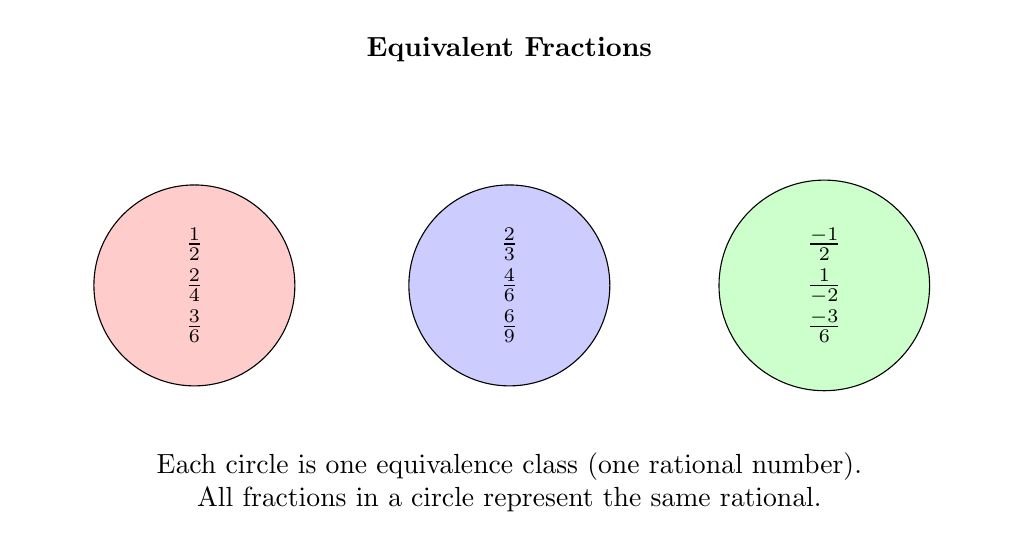
\begin{tikzpicture}[scale=1.0]
    \node at (5, 5) {\textbf{Equivalent Fractions}};
    
    % Circles showing fraction equivalence classes
    \node[circle, draw, fill=red!20, inner sep=10pt] (f1) at (1, 2) {
        \begin{tabular}{c}
            $\frac{1}{2}$ \\[0.1cm]
            $\frac{2}{4}$ \\[0.1cm]
            $\frac{3}{6}$
        \end{tabular}
    };
    
    \node[circle, draw, fill=blue!20, inner sep=10pt] (f2) at (5, 2) {
        \begin{tabular}{c}
            $\frac{2}{3}$ \\[0.1cm]
            $\frac{4}{6}$ \\[0.1cm]
            $\frac{6}{9}$
        \end{tabular}
    };
    
    \node[circle, draw, fill=green!20, inner sep=10pt] (f3) at (9, 2) {
        \begin{tabular}{c}
            $\frac{-1}{2}$ \\[0.1cm]
            $\frac{1}{-2}$ \\[0.1cm]
            $\frac{-3}{6}$
        \end{tabular}
    };
    
    \node[below, text width=12cm, align=center] at (5, 0) {
        Each circle is one equivalence class (one rational number). \\
        All fractions in a circle represent the same rational.
    };
\end{tikzpicture}
\end{center}

\subsection{Arithmetic on $\mathbb{Q}$}

\begin{definition}[Operations on $\mathbb{Q}$]
Define addition, multiplication, and inversion:

\textbf{Addition}: $\frac{p}{q} + \frac{r}{s} := \frac{ps + qr}{qs}$

\textbf{Multiplication}: $\frac{p}{q} \cdot \frac{r}{s} := \frac{pr}{qs}$

\textbf{Negation}: $-\frac{p}{q} := \frac{-p}{q}$

\textbf{Reciprocal}: If $p \neq 0$, then $\left(\frac{p}{q}\right)^{-1} := \frac{q}{p}$

\textbf{Embedding}: $\iota: \mathbb{Z} \to \mathbb{Q}$ by $\iota(n) = \frac{n}{1}$
\end{definition}

\begin{theorem}
Addition on $\mathbb{Q}$ is well-defined.
\end{theorem}

\begin{proof}
Suppose $\frac{p}{q} = \frac{p'}{q'}$ and $\frac{r}{s} = \frac{r'}{s'}$.

Then $(p, q) \sim (p', q')$ and $(r, s) \sim (r', s')$, which means:
\[pq' = qp' \quad \text{and} \quad rs' = sr'\]

We need to show:
\[\frac{ps + qr}{qs} = \frac{p's' + q'r'}{q's'}\]

That is, $(ps + qr, qs) \sim (p's' + q'r', q's')$, which means:
\[(ps + qr)(q's') = (p's' + q'r')(qs)\]

\textbf{Expand the left side:}
\[(ps + qr)(q's') = psq's' + qrq's' = ps \cdot q's' + qr \cdot q's'\]

\textbf{Expand the right side:}
\[(p's' + q'r')(qs) = p's'qs + q'r'qs = p's' \cdot qs + q'r' \cdot qs\]

\textbf{Compare terms:}

For the first terms: $ps \cdot q's' = p's' \cdot qs$

Using $pq' = qp'$, multiply both sides by $ss'$:
\[pq'ss' = qp'ss'\]
\[ps \cdot q's' = p's \cdot qs\]

But wait, we need $ps \cdot q's' = p's' \cdot qs$. Multiply $pq' = qp'$ by $ss'$:
\[pq'ss' = qp'ss'\]

Rearranging: $ps \cdot s'q' = s'p' \cdot qs$, so $ps \cdot q's' = p's' \cdot qs$. $\checkmark$

For the second terms: $qr \cdot q's' = q'r' \cdot qs$

Using $rs' = sr'$, multiply both sides by $qq'$:
\[rs'qq' = sr'qq'\]
\[qr \cdot q's' = qs \cdot q'r'\]

Therefore $qr \cdot q's' = q'r' \cdot qs$. $\checkmark$

Adding both verified equations:
\[ps \cdot q's' + qr \cdot q's' = p's' \cdot qs + q'r' \cdot qs\]
\[(ps + qr)(q's') = (p's' + q'r')(qs)\]

Therefore addition is well-defined. $\checkmark$
\end{proof}

\begin{theorem}
Multiplication on $\mathbb{Q}$ is well-defined.
\end{theorem}

\begin{proof}
Suppose $\frac{p}{q} = \frac{p'}{q'}$ and $\frac{r}{s} = \frac{r'}{s'}$.

Then $pq' = qp'$ and $rs' = sr'$.

We need to show:
\[\frac{pr}{qs} = \frac{p'r'}{q's'}\]

That is, $(pr)(q's') = (p'r')(qs)$.

\textbf{Expand:}
\[(pr)(q's') = prq's' = p(rs')q' = p(sr')q' \quad \text{(using $rs' = sr'$)}\]
\[= ps \cdot r'q' = ps \cdot q'r'\]

But from $pq' = qp'$, multiply by $sr'$:
\[pq'sr' = qp'sr'\]
\[ps \cdot q'r' = qp' \cdot sr' = qp' \cdot rs' \quad \text{(using $sr' = rs'$)}\]
\[= q(p'r')s = (p'r')(qs)\]

Therefore $(pr)(q's') = (p'r')(qs)$, so multiplication is well-defined. $\checkmark$
\end{proof}

\begin{theorem}[Properties of $\mathbb{Q}$]
$(\mathbb{Q}, +, \cdot, 0, 1)$ is a \textbf{field}:
\begin{enumerate}
    \item $(\mathbb{Q}, +)$ is an abelian group with identity $0 = \frac{0}{1}$
    \item $(\mathbb{Q} \setminus \{0\}, \cdot)$ is an abelian group with identity $1 = \frac{1}{1}$
    \item Distributivity: $a(b + c) = ab + ac$
\end{enumerate}
\end{theorem}

\begin{proof}[Proof Sketch]
Most properties follow from $\mathbb{Z}$ being an integral domain.

\textbf{Key new property}: Every non-zero element has a multiplicative inverse:
\[\frac{p}{q} \cdot \frac{q}{p} = \frac{pq}{qp} = \frac{pq}{pq} = \frac{1}{1} = 1\]

(This requires $p \neq 0$, which is guaranteed for $\frac{p}{q} \neq 0$.)

Therefore $\mathbb{Q}$ is a field. $\checkmark$
\end{proof}

\begin{example}[Division in $\mathbb{Q}$]
Now we can define division:
\[\frac{a}{b} \div \frac{c}{d} := \frac{a}{b} \cdot \left(\frac{c}{d}\right)^{-1} = \frac{a}{b} \cdot \frac{d}{c} = \frac{ad}{bc}\]

For example:
\[\frac{2}{3} \div \frac{4}{5} = \frac{2}{3} \cdot \frac{5}{4} = \frac{10}{12} = \frac{5}{6}\]
\end{example}

\section{Summary: The Tower of Number Systems}

\begin{center}
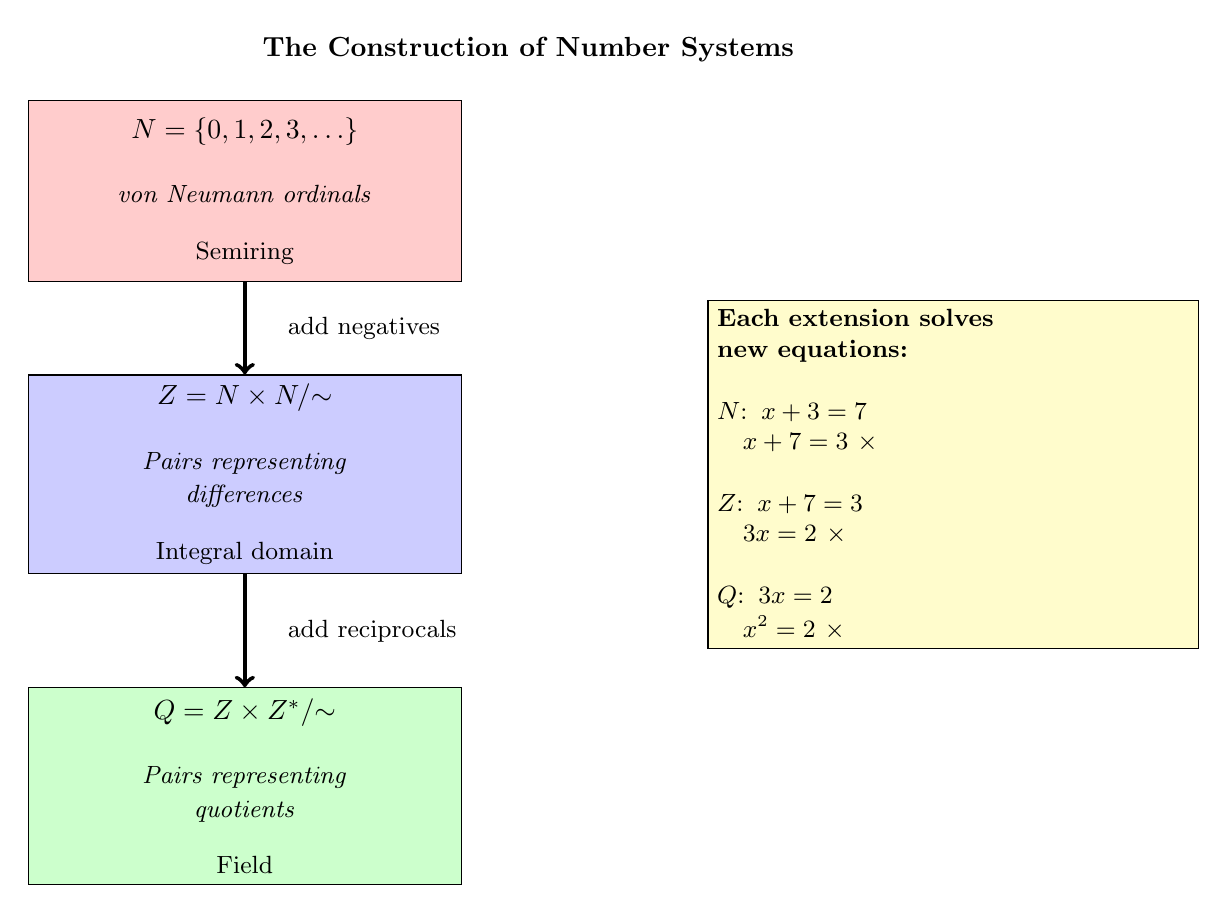
\begin{tikzpicture}[scale=1.2]
    \node at (6, 6) {\textbf{The Construction of Number Systems}};
    
    % Natural numbers
    \node[rectangle, draw, fill=red!20, minimum width=5.5cm, minimum height=2.3cm, align=center] (N) at (3, 4.5) {
        $\mathbb{N} = \{0, 1, 2, 3, \ldots\}$ \\[0.4cm]
        \small\textit{von Neumann ordinals} \\[0.3cm]
        \small Semiring
    };
    
    % Integers
    \node[rectangle, draw, fill=blue!20, minimum width=5.5cm, minimum height=2.5cm, align=center] (Z) at (3, 1.5) {
        $\mathbb{Z} = \mathbb{N} \times \mathbb{N} / {\sim}$ \\[0.4cm]
        \small\textit{Pairs representing} \\
        \small\textit{differences} \\[0.3cm]
        \small Integral domain
    };
    
    % Rationals
    \node[rectangle, draw, fill=green!20, minimum width=5.5cm, minimum height=2.5cm, align=center] (Q) at (3, -1.8) {
        $\mathbb{Q} = \mathbb{Z} \times \mathbb{Z}^* / {\sim}$ \\[0.4cm]
        \small\textit{Pairs representing} \\
        \small\textit{quotients} \\[0.3cm]
        \small Field
    };
    
    % Arrows
    \draw[->, ultra thick] (N.south) -- (Z.north) node[midway, right=0.4cm] {\small add negatives};
    \draw[->, ultra thick] (Z.south) -- (Q.north) node[midway, right=0.4cm] {\small add reciprocals};
    
    % Properties box
    \node[rectangle, draw, fill=yellow!20, text width=6cm, align=left] at (10.5, 1.5) {
        \small\textbf{Each extension solves} \\
        \small\textbf{new equations:} \\[0.4cm]
        \small $\mathbb{N}$: $x + 3 = 7$ \checkmark \\
        \small \quad $x + 7 = 3$ $\times$ \\[0.4cm]
        \small $\mathbb{Z}$: $x + 7 = 3$ \checkmark \\
        \small \quad $3x = 2$ $\times$ \\[0.4cm]
        \small $\mathbb{Q}$: $3x = 2$ \checkmark \\
        \small \quad $x^2 = 2$ $\times$
    };
\end{tikzpicture}
\end{center}

\begin{keyidea}
\textbf{The Pattern of Extension}:

\begin{enumerate}
    \item Start with structure $A$ (e.g., $\mathbb{N}$)
    \item Identify limitation (e.g., no negative numbers)
    \item Form pairs $A \times A$ (or similar)
    \item Define equivalence relation capturing desired property
    \item Quotient by equivalence: $B = (A \times A) / {\sim}$
    \item Define operations on $B$ that extend operations on $A$
    \item Prove $B$ has desired properties (ring, field, etc.)
    \item Embed $A \hookrightarrow B$ as a substructure
\end{enumerate}

This pattern works for:
\begin{itemize}
    \item $\mathbb{N} \to \mathbb{Z}$ (add additive inverses)
    \item $\mathbb{Z} \to \mathbb{Q}$ (add multiplicative inverses)
    \item $\mathbb{Q} \to \mathbb{R}$ (add limits, via Dedekind cuts or Cauchy sequences)
    \item $\mathbb{R} \to \mathbb{C}$ (add square roots of negatives)
\end{itemize}

This is the systematic way modern mathematics builds everything from sets!
\end{keyidea}

\section{Looking Forward: The Real Numbers}

\begin{intuition}
Rationals are still insufficient: $x^2 = 2$ has no solution in $\mathbb{Q}$.

The real numbers $\mathbb{R}$ fill the ``gaps'' in $\mathbb{Q}$:

\textbf{Dedekind Cuts} (1872): A real number is a partition of $\mathbb{Q}$ into ``left'' and ``right'' parts.

\textbf{Cauchy Sequences} (1872): A real number is an equivalence class of converging sequences of rationals.

Both constructions are long and technical, requiring limits and completeness axioms.

For now, we've completed the construction $\mathbb{N} \to \mathbb{Z} \to \mathbb{Q}$ entirely from set theory!
\end{intuition}

\begin{remark}
The construction of $\mathbb{R}$ from $\mathbb{Q}$ is typically covered in real analysis courses. The key ideas:

\textbf{Dedekind Cut}: A cut $(L, R)$ where:
\begin{itemize}
    \item $L \cup R = \mathbb{Q}$, $L \cap R = \emptyset$
    \item $L$ has no maximum, $R$ has no minimum
    \item $\forall \ell \in L, \forall r \in R, \ell < r$
\end{itemize}

Examples:
\begin{itemize}
    \item $\sqrt{2} = (\{q \in \mathbb{Q} : q < 0 \text{ or } q^2 < 2\}, \{q \in \mathbb{Q} : q > 0 \text{ and } q^2 > 2\})$
    \item $\pi = (\{q \in \mathbb{Q} : q < \pi\}, \{q \in \mathbb{Q} : q > \pi\})$ (requires defining $\pi$ first!)
\end{itemize}

This construction ensures $\mathbb{R}$ is \textbf{complete}: every Cauchy sequence converges, every bounded set has a supremum.
\end{remark}

\section{Conclusion}

\begin{center}
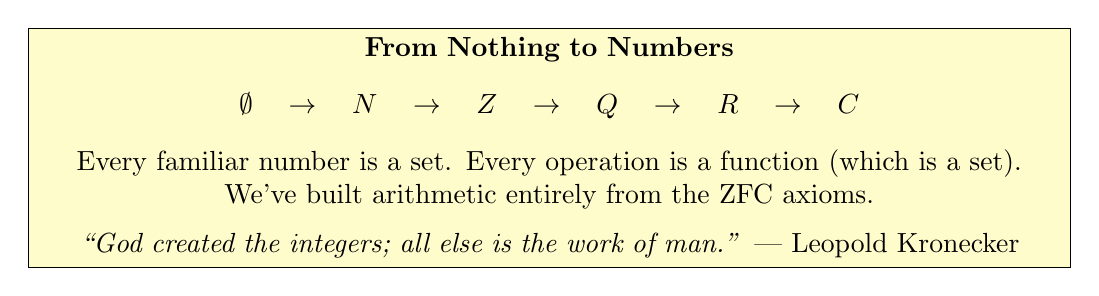
\begin{tikzpicture}[scale=1.0]
    \node[rectangle, draw, fill=yellow!20, text width=13cm, align=center] at (6.5,0) {
    \textbf{From Nothing to Numbers} \\[0.3cm]
    $\emptyset \to \mathbb{N} \to \mathbb{Z} \to \mathbb{Q} \to \mathbb{R} \to \mathbb{C}$ \\[0.3cm]
    Every familiar number is a set. Every operation is a function (which is a set). \\
    We've built arithmetic entirely from the ZFC axioms. \\[0.2cm]
    \textit{``God created the integers; all else is the work of man.''} --- Leopold Kronecker
    };
\end{tikzpicture}
\end{center}

\begin{historicalnote}
This construction answers Dedekind's question: \textit{``What are numbers and what should they be?''}

\textbf{Answer}: Numbers are equivalence classes of pairs of simpler numbers, all the way down to sets.

This is the crowning achievement of 19th-century rigor:
\begin{itemize}
    \item Mathematics is \textit{derivable} from logic and set theory
    \item No appeals to intuition or physical reality are needed
    \item Every theorem traces back to axioms through pure deduction
\end{itemize}

But Gödel (1931) showed limits: No system can prove all truths about arithmetic. Some statements are forever undecidable.

Nevertheless, the ZFC construction of number systems remains the standard foundation of modern mathematics.
\end{historicalnote}
